\documentclass[12pt, twoside, openany]{book}
%\documentclass[12pt, oneside]{book}  % single-sided printing

% page margins
\usepackage[a4paper,top=2.5cm,bottom=2.5cm,left=3.5cm,right=2cm]{geometry}
% UTF-8 font encoding
\usepackage[utf8]{inputenc}
\usepackage[T1]{fontenc}

% English thesis - babel for Slovak disabled
%\usepackage[slovak]{babel}

% line spacing per university guidelines
\linespread{1.25} % 1.25 corresponds to 1.5 line spacing

% source code listings
\usepackage{listings}
\renewcommand{\lstlistingname}{Listing}
\lstset{frame=lines}

% graphics
\usepackage{graphicx}
% include full PDF pages (for thesis assignment)
\usepackage{pdfpages}
% proper URL formatting
\usepackage{url}
% hyperlinks within the document
\usepackage[hidelinks,breaklinks]{hyperref}


% -------------------
% --- Basic definitions
% -------------------
\def\mfrok{2026}
\def\mfnazov{WebTransport Protocol Fuzzing}
\def\mftyp{Bachelor Thesis}
\def\mfautor{Vladyslav Havriuk}
\def\mfskolitel{doc. RNDr. Martin Stanek, PhD.}

%\def\mfkonzultant{tit. Name Surname, tit. }

\def\mfmiesto{Bratislava, \mfrok}

\def\mfodbor{Computer Science}
\def\program{Computer Science}

\def\mfpracovisko{ Department of Computer Science }

\begin{document}     
\frontmatter
\pagestyle{empty}

% -------------------
% --- Cover page ------
% -------------------

\begin{center}
\sc\large
Comenius University in Bratislava\\
Faculty of Mathematics, Physics and Informatics

\vfill

{\LARGE\mfnazov}\\
\mftyp
\end{center}

\vfill

{\sc\large 
\noindent \mfrok\\
\mfautor
}

\cleardoublepage
% --- end of cover page ----

% -------------------
% --- Title page
% -------------------

\noindent

\begin{center}
\sc  
\large
Comenius University in Bratislava\\
Faculty of Mathematics, Physics and Informatics

\vfill

{\LARGE\mfnazov}\\
\mftyp
\end{center}

\vfill

\noindent
\begin{tabular}{ll}
Study Programme: & \program \\
Field of Study: & \mfodbor \\
Department: & \mfpracovisko \\
Supervisor: & \mfskolitel \\
% Consultant: & \mfkonzultant \\
\end{tabular}

\vfill


\noindent \mfmiesto\\
\mfautor

\cleardoublepage
% --- End of title page


% -------------------
% --- Thesis assignment from AIS
% -------------------
% Thesis assignment from AIS

\newpage
\setcounter{page}{3}
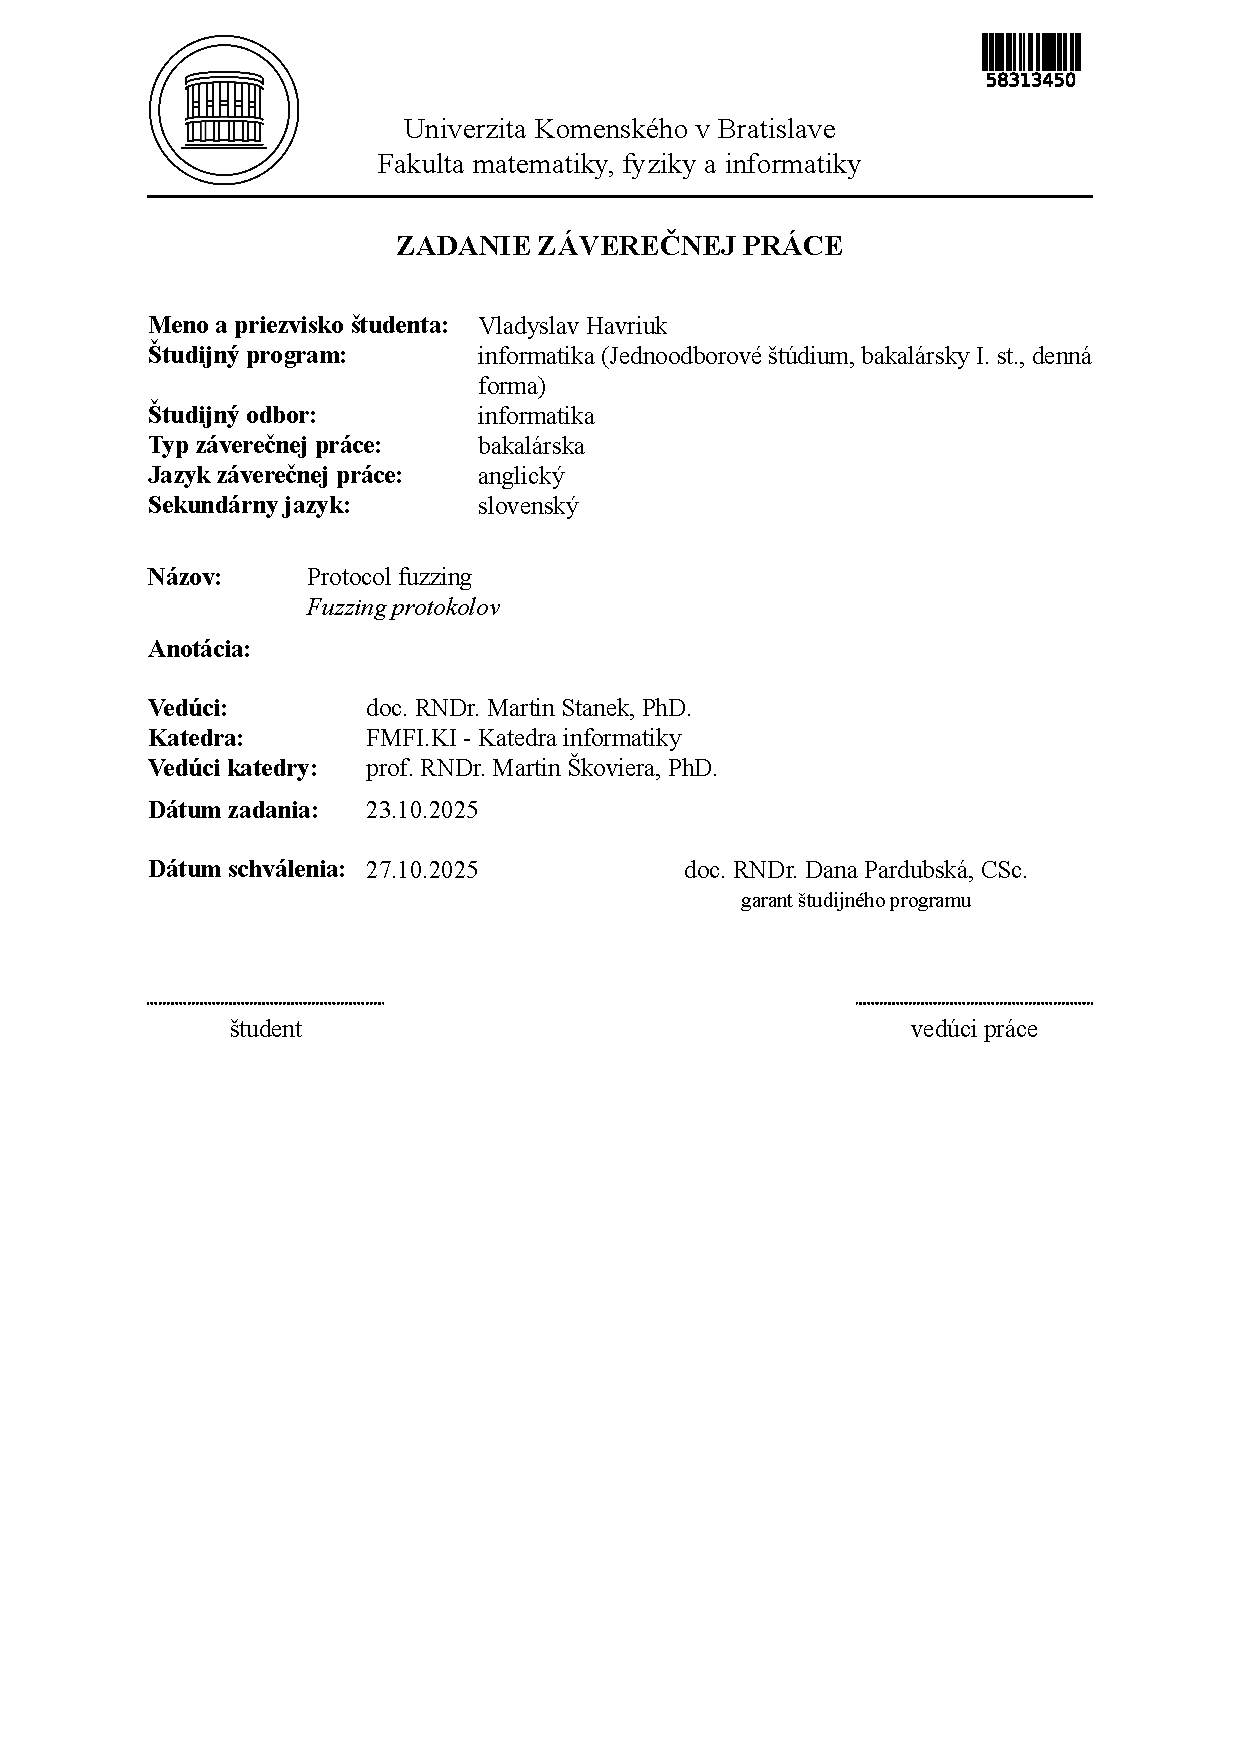
\includepdf{images/zadanie-en.pdf}

% --- End of assignment


% -------------------
%   Declaration and optional acknowledgments
% -------------------
\newpage
\pagestyle{plain}
\paragraph{Declaration:}
I hereby declare that I have independently written this entire
bachelor thesis entitled ``\mfnazov'', including all its
figures and appendices, using the literature listed in the attached
bibliography.

% Uveďte na čo ste nástroje používali
% Podľa typu použitia potom nástroje aj citujte v texte
In preparation of the thesis I have also used the following artificial
intelligence tools: OpenCode and Anthropic Claude for the following
purposes: implementing some of the code segments, and minor editing and
formatting of thesis text. I
have used artificial intelligence tools in accordance with relevant
legal regulations, academic rights and freedoms, ethical and moral
principles while simultaneously maintaining academic integrity. I am
aware that I am fully responsible for the accuracy of the final text.

\paragraph{Acknowledgments:} I would like to thank my supervisor doc. RNDr. Martin Stanek, PhD. for his expert guidance, valuable advice, and comments during the preparation of this thesis.

% --- End of acknowledgments

% -------------------
%   Abstract - Slovak
% -------------------
\newpage 
\section*{Abstrakt}

Fuzzing protokolov je technika pou\v{z}\'{i}van\'{a} na testovanie implement\'{a}ci\'{i} protokolov. Bola \'{u}spe\v{s}ne pou\v{z}it\'{a} na identifik\'{a}ciu implementa\v{c}n\'{y}ch ch\'{y}b a bezpe\v{c}nostn\'{y}ch zranite\v{l}nost\'{i} v r\^{o}znych protokoloch. Cie\v{l}om tejto pr\'{a}ce je presk\'{u}ma\v{t} met\'{o}dy fuzzingu protokolov a aplikova\v{t} ich na re\'{a}lne implement\'{a}cie protokolu WebTransport. V\'{y}sledky s\'{u} analyzovan\'{e} a diskutovan\'{e}.

T\'{a}to pr\'{a}ca sa zaober\'{a} fuzzingom protokolov na identifik\'{a}ciu ch\'{y}b v implement\'{a}ci\'{a}ch a zranite\v{l}nost\'{i}. Predstavujeme vyvinut\'{y} fuzzer zalo\v{z}en\'{y} na BooFuzz pre protokol WebTransport, ktor\'{y} zah\v{r}\v{n}a mut\'{a}cie \v{s}trukt\'{u}ry spr\'{a}v a duplik\'{a}ciu sekvenci\'{i}. Pr\'{i}spevok spo\v{c}\'{i}va v integr\'{a}cii s aioquic pre QUIC podporu, testovan\'{i} na echo serveroch a anal\'{y}ze v\'{y}sledkov, vr\'{a}tane objavenia chyby v Rust kni\v{z}nici. V\'{y}sledky ukazuj\'{u} efektivitu pr\'{i}stupu v odha\v{l}ovan\'{i} pan\'{i}k v pracovn\'{y}ch vl\'{a}knach, prispieva\-j\'{u}c k spo\v{l}ahlivosti WebTransportu.

\paragraph*{K\v{l}\'{u}\v{c}ov\'{e} slov\'{a}:} fuzzing, WebTransport, QUIC, HTTP/3, testovanie protokolov, bezpe\v{c}nos\v{t}
% --- End of Slovak abstract


% -------------------
% --- Abstract - English 
% -------------------
\newpage 
\section*{Abstract}

Protocol fuzzing is a technique used to test protocol implementations. It has been successfully employed to identify implementation errors and security vulnerabilities in various protocols. The goal of this thesis is to explore methods of protocol fuzzing and apply them to real-world implementations of the WebTransport protocol. The results are analyzed and discussed.

This thesis addresses protocol fuzzing for identifying bugs in implementations and vulnerabilities. We present a developed fuzzer based on BooFuzz for the WebTransport protocol, which includes message structure mutations and sequence duplication. The contribution lies in the integration with aioquic for QUIC support, testing on echo servers, and analysis of results, including the discovery of a bug in a Rust library. The results demonstrate the effectiveness of the approach in detecting worker thread panics, contributing to the reliability of WebTransport.

\paragraph*{Keywords:} fuzzing, WebTransport, QUIC, HTTP/3, protocol testing, security

% --- End of English abstract

% -------------------
% --- Table of contents
% -------------------

\cleardoublepage

\tableofcontents

% ---  End of table of contents

% -------------------
% --- Lists of figures, tables - optional
% -------------------

\newpage 

\listoffigures
\listoftables

% ---  End of lists

\mainmatter
\pagestyle{headings}


\input intro.tex 

\input related_work.tex

\input methodology.tex

\input results.tex

\input conclusion.tex

% -------------------
% --- Bibliography
% -------------------


\newpage	

\backmatter

\thispagestyle{empty}
\clearpage
\addcontentsline{toc}{chapter}{References}
\bibliographystyle{plain}
\bibliography{literatura} 

%---end of references

% -------------------
%--- Appendices---
% -------------------

\input appendixA-en.tex

\end{document}
